% Geant4 Physics Manual Entry
%
% Use 'make' to run latex and generate the pdf file
%
% Doug Wright

\documentclass[11pt]{article}
\usepackage{h4}

\newcommand{\notgeant}[1]{}% exclude some things from the geant manual

%\ucrl{UCRL-AR-228518}

\begin{document}

\section{Fission with improved multiplicity sampling}

As an alternative to the fission model described in the previous
section there is a modified model that produces more accurate
multiplicity distributions for the emitted neutrons and gamma rays
from spontaneous and neutron-induced fission. This was motivated by
detailed statistical studies of fission chains in multiplying
media. This model is data-driven and incorporates all available
multiplicity measurements found in the literature. Empirical models
are employed whenever multiplicity data are not available.
Essentially no data are available for the correlations between the
neutrons and gammas, so this model samples these distributions
independently. By default, this model effectively scales the
multiplicity data to match the average multiplicity value
($\bar{\nu}$) found in the GEANT4 evaluated data library. Therefore,
only isotopes that have a measured $\bar{\nu}$ in the data library
will emit fission gammas or neutrons. At present the gammas and
neutrons are emitted isotropically. The data and empirical models are
described in detail in the following subsections.

\section{Spontaneous fission and neutron-induced fission\label{neutrons}}

\subsection{Neutron number distribution}\label{sec:neutron number distribution}

Based on reasonable assumptions about the distribution of excitation
energy among fission fragments, Terrell~\cite{Terrell 1957} showed
that the probability P$_\nu$ of observing $\nu$ neutrons from fission
can be approximated by a Gaussian-like distribution
\begin{equation}
\sum_{n=0}^{\nu}P_n = \frac{1}{2\pi}\int_{-\infty}^{\frac{\nu-\bar{\nu} 
                    + \frac{1}{2}+b}{\sigma}}e^{-\frac{t^2}{2}dt}
\end{equation}
where $\bar{\nu}$ is the average number of neutrons, $\sigma$ (set to
1.079) is the width of the distribution, and $b$ is a small correction
factor ($b<0.01$) that ensures that the discrete probability
distribution has the correct average $\bar{\nu}$. This model is used
when no explicit multiplicity data are available.

\subsubsection*{Neutron-induced fission data}

Zucker and Holden~\cite{Zucker and Holden 1986} measured the neutron
multiplicity distributions for $^{235}$U, $^{238}$U, and $^{239}$Pu
(see Tables~\ref{Neutron number distribution for induced fission in
235U}-\ref{Neutron number distribution for induced fission in 239Pu}),
as a function of the incident neutron energy $E_n$ from 
zero through ten MeV in increments of one MeV.  Fig.~\ref{235U induced
fission 6MeV} shows the neutron number distribution for induced
fission of $^{235}$U. Gwin, Spencer and Ingle~\cite{Gwin 1984}
measured the distribution at thermal energies for $^{235}$U. In
addition, there are many measurements of $\bar{\nu}$, the average
number of emitted neutrons, for many isotopes. Since there are multiple
methods for parameterizing the multiplicity data and 
renormalizing the overall distributions to agree with the specific measured
values of $\bar{\nu}$, we provide four options for generating 
neutron multiplicity distributions. 
\notgeant{These options are selected by the internal variable {\tt nudist}, default=3.}

\begin{table}[ht]
\footnotesize
\begin{center}
\begin{tabular}{|c|cccccccc|c|} \hline
$E_n$ & $\nu$=0 & 1 & 2 & 3 & 4 & 5 & 6 & 7 & $\bar{\nu}$ \\ \hline
0 & .0317223 & .1717071 & .3361991 & .3039695 & .1269459 & .0266793 & .0026322 & .0001449 & 2.4140000 \\
1 & .0237898 & .1555525 & .3216515 & .3150433 & .1444732 & .0356013 & .0034339 & .0004546 & 2.5236700 \\
2 & .0183989 & .1384891 & .3062123 & .3217566 & .1628673 & .0455972 & .0055694 & .0011093 & 2.6368200 \\
3 & .0141460 & .1194839 & .2883075 & .3266568 & .1836014 & .0569113 & .0089426 & .0019504 & 2.7623400 \\
4 & .0115208 & .1032624 & .2716849 & .3283426 & .2021206 & .0674456 & .0128924 & .0027307 & 2.8738400 \\
5 & .0078498 & .0802010 & .2456595 & .3308175 & .2291646 & .0836912 & .0187016 & .0039148 & 3.0386999 \\
6 & .0046272 & .0563321 & .2132296 & .3290407 & .2599806 & .1045974 & .0265604 & .0056322 & 3.2316099 \\
7 & .0024659 & .0360957 & .1788634 & .3210507 & .2892537 & .1282576 & .0360887 & .0079244 & 3.4272800 \\
8 & .0012702 & .0216090 & .1472227 & .3083032 & .3123950 & .1522540 & .0462449 & .0107009 & 3.6041900 \\
9 & .0007288 & .0134879 & .1231200 & .2949390 & .3258251 & .1731879 & .0551737 & .0135376 & 3.7395900 \\
10& .0004373 & .0080115 & .1002329 & .2779283 & .3342611 & .1966100 & .0650090 & .0175099 & 3.8749800 \\ \hline
\end{tabular}
\end{center}
\caption{Neutron number distribution for induced fission in $^{235}$U.}
\label{Neutron number distribution for induced fission in 235U}
\end{table}

\begin{table}[ht]
\footnotesize
\begin{center}
\begin{tabular}{|c|ccccccccc|c|} \hline
$E_n$ & $\nu$=0 & 1 & 2 & 3 & 4 & 5 & 6 & 7 & 8 & $\bar{\nu}$ \\ \hline
0 & .0396484 & .2529541 & .2939544 & .2644470 & .1111758 & .0312261 & .0059347 & .0005436 & .0001158 & 2.2753781 \\
1 & .0299076 & .2043215 & .2995886 & .2914889 & .1301480 & .0363119 & .0073638 & .0006947 & .0001751 & 2.4305631 \\
2 & .0226651 & .1624020 & .2957263 & .3119098 & .1528786 & .0434233 & .0097473 & .0009318 & .0003159 & 2.5857481 \\
3 & .0170253 & .1272992 & .2840540 & .3260192 & .1779579 & .0526575 & .0130997 & .0013467 & .0005405 & 2.7409331 \\
4 & .0124932 & .0984797 & .2661875 & .3344938 & .2040116 & .0640468 & .0173837 & .0020308 & .0008730 & 2.8961181 \\
5 & .0088167 & .0751744 & .2436570 & .3379711 & .2297901 & .0775971 & .0225619 & .0030689 & .0013626 & 3.0513031 \\
6 & .0058736 & .0565985 & .2179252 & .3368863 & .2541575 & .0933127 & .0286200 & .0045431 & .0031316 & 3.2064881 \\
7 & .0035997 & .0420460 & .1904095 & .3314575 & .2760413 & .1112075 & .0355683 & .0065387 & .0031316 & 3.3616731 \\
8 & .0019495 & .0309087 & .1625055 & .3217392 & .2943792 & .1313074 & .0434347 & .0091474 & .0046284 & 3.5168581 \\
9 & .0008767 & .0226587 & .1356058 & .3076919 & .3080816 & .1536446 & .0522549 & .0124682 & .0067176 & 3.6720432 \\
10& .0003271 & .0168184 & .1111114 & .2892434 & .3160166 & .1782484 & .0620617 & .0166066 & .0095665 & 3.8272281 \\ \hline
\end{tabular}
\end{center}
\caption{Neutron number distribution for induced fission in $^{238}$U.}
\label{Neutron number distribution for induced fission in 238U}
\end{table}

\begin{table}[ht]
\footnotesize
\begin{center}
\begin{tabular}{|c|ccccccccc|c|} \hline
$E_n$ & $\nu$=0 & 1 & 2 & 3 & 4 & 5 & 6 & 7 & 8 & $\bar{\nu}$ \\ \hline
0 & .0108826 & .0994916 & .2748898 & .3269196 & .2046061 & .0726834 & .0097282 & .0006301 & .0001685 & 2.8760000 \\
1 & .0084842 & .0790030 & .2536175 & .3289870 & .2328111 & .0800161 & .0155581 & .0011760 & .0003469 & 3.0088800 \\
2 & .0062555 & .0611921 & .2265608 & .3260637 & .2588354 & .0956070 & .0224705 & .0025946 & .0005205 & 3.1628300 \\
3 & .0045860 & .0477879 & .1983002 & .3184667 & .2792811 & .1158950 & .0301128 & .0048471 & .0007233 & 3.3167800 \\
4 & .0032908 & .0374390 & .1704196 & .3071862 & .2948565 & .1392594 & .0386738 & .0078701 & .0010046 & 3.4707300 \\
5 & .0022750 & .0291416 & .1437645 & .2928006 & .3063902 & .1641647 & .0484343 & .0116151 & .0014149 & 3.6246800 \\
6 & .0014893 & .0222369 & .1190439 & .2756297 & .3144908 & .1892897 & .0597353 & .0160828 & .0029917 & 3.7786300 \\
7 & .0009061 & .0163528 & .0968110 & .2558524 & .3194566 & .2134888 & .0729739 & .0213339 & .0020017 & 3.9325800 \\
8 & .0004647 & .0113283 & .0775201 & .2335926 & .3213289 & .2356614 & .0886183 & .0274895 & .0039531 & 4.0865300 \\
9 & .0002800 & .0071460 & .0615577 & .2089810 & .3200121 & .2545846 & .1072344 & .0347255 & .0054786 & 4.2404900 \\
10& .0002064 & .0038856 & .0492548 & .1822078 & .3154159 & .2687282 & .1295143 & .0432654 & .0075217 & 4.3944400 \\ \hline
\end{tabular}
\end{center}
\caption{Neutron number distribution for induced fission in $^{239}$Pu.}
\label{Neutron number distribution for induced fission in 239Pu}
\end{table}

\begin{figure}[ht]
\begin{center}
\includegraphics[scale=0.4, angle=-90]{eps/U235_6MeV_nudist.eps}
\end{center}
\caption{Induced fission in $^{235}$U, incident neutron energy = 6MeV}
\label{235U induced fission 6MeV}
\end{figure}

The first option\notgeant{ ({\tt nudist=0})} uses a fit to the Zucker
and Holden data \cite{Zucker and Holden 1986} by
Valentine~\cite{Valentine 1996,Valentine 2000}. Valentine
expressed the P$_{\nu}$'s (for $\nu=0$, ..., 8) as 5$^{th}$ order
polynomials in $E_n$, the incident neutron energy. These functions 
P$_{\nu}(E_n)$ are used to sample the neutron multiplicity for 
$E_n$ in the range 0 to 10 MeV.  When $E_n$ is greater than 10 MeV, 
$E_n$=10 MeV is used to generate P$_{\nu}$.

In addition to using the Zucker and Holden data above for incident
neutron energies $E_n$ above 1 MeV, the second
option\notgeant{ ({\tt nudist=1})} also uses the Gwin, Spencer and
Ingle data~\cite{Gwin 1984} for $^{235}$U at thermal energies (0 MeV) 
to generate P$_{\nu}(E_n)$ polynomials. As in the first option, when
$E_n$ is greater than 10 MeV, $E_n$=10 MeV is used to generate
P$_{\nu}$.

The third option\notgeant{ ({\tt nudist=2})} implements an alternative
polynomial fit from Valentine ~\cite{Valentine 2000} of  P$_{\nu}$
as a function of $\bar{\nu}$ instead of $E_n$.
%
%{\it"A unique
%relationship P$_{\nu}(\bar{\nu})$ can sufficiently
%well capture the multiplicity distributions of a number of major
%isotopes. This distribution is expressed as a function of the average
%number of neutrons emitted $\bar{\nu}$.}" 
%
When a neutron induces a fission, the algorithm converts the incident
neutron energy $E_n$ into $\bar{\nu}$ using conversion tables
(typically ENDF/EDNL), generates the P$_{\nu}$ distributions for that
value of $\bar{\nu}$, and then samples the P$_{\nu}$ distributions to
determine $\nu$. Following a suggestion of Frehaut~\cite{Frehaut 1988},
the least-square fits to the $^{235}$U data are used for both $^{235}$U 
and $^{233}$U neutron induced fission, the fits to $^{238}$U are used 
for $^{232}$U, $^{234}$U, $^{236}$U and $^{238}$U, while the fits to 
$^{239}$Pu are used for $^{239}$Pu and $^{241}$Pu. Data come from
Zucker and Holden. For $^{235}$U, data comes from Zucker and Holden 
for $E_n$ greater than 1 MeV, and Gwin, Spencer and
Ingle for 0 MeV. The fits are only used when $\bar{\nu}$ is in the 
range of the $\bar{\nu}$'s for the tabulated data. Otherwise, 
Terrell's approximation is used.

The fourth option, which is the default\notgeant{ ({\tt nudist=3})},
is similar to the third option except that the P$_{\nu}$ distributions
are not functions of $\bar{\nu}$, but are left intact as multiplicity
distributions for the data listed in Gwin, Spencer and
Ingle, and for the data listed in Zucker and
Holden. The multiplicity distribution P$_{\nu}$ from which the number
of neutrons will be sampled is selected based on the value of
$\bar{\nu}$ for a given induced fission event.  For instance, if
P$_{\nu}(1\ \mathrm{MeV})$ has $\bar{\nu}=2.4$, P$_{\nu}(2\ \mathrm{MeV})$ has
$\bar{\nu}=2.6$, and $\bar{\nu}$ is 2.45 at the energy of the incident
fission-inducing neutron (this value $\bar{\nu}$ comes typically from
cross-section data libraries such and ENDF/ENDL), the probability of
sampling the number of neutrons ${\nu}$ from P$_{\nu}(1\ \mathrm{MeV})$ and
P$_{\nu}(2\ \mathrm{MeV})$ will be 75\% and 25\%, respectively. This technique
is only used when $\bar{\nu}$ is in the range of the $\bar{\nu}$'s for
the tabulated data. Otherwise, Terrell's approximation is used.  This
last way of computing ${\nu}$ has several advantages: first, the data
as listed in the original papers is used exactly, as opposed to
approximated by low-ordered polynomials least-square fitting the
original data. Second, the data from the Gwin, Spencer and
Ingle paper, and the data from the Zucker and Holden paper is
entered as-is as a table in the code, and can easily be checked and
maintained if necessary by the application developer. Third the method
provides a simple and statistically correct mechanism of sampling the
data tables. \notgeant{The fission module behaves in this
manner when the 'nudist' option is set to 3, which is also the default
behavior.}

\subsubsection*{Spontaneous fission data}

Table~\ref{Neutron number distribution for spontaneous fission} summarizes
the spontaneous fission neutron number distributions for several isotopes,
along with their references~\cite{Holden and Zucker BNL,Santi 2005,
BNL-36467,Dakavoski 1973,Hoffman 1980,Lazarev 1974}. For $^{252}$Cf, the 
fission module can be set to use either the measurements by 
Spencer~\cite{Spencer 1982}\notgeant{ ({\tt ndist=0})}, which is the 
default, or Boldeman~\cite{Boldeman 1985}\notgeant{ ({\tt ndist=1})}.
For $^{246}$Cm, $^{248}$Cm, $^{246}$Cf, $^{250}$Cf, $^{254}$Cf, $^{257}$Fm 
and $^{252}$No, the Watt parameters are not available, so even though the 
number of spontaneous fission neutrons could be sampled, no energy could be 
attributed to them, and the fission library module thus fails for these
7 nuclides.

\begin{table}[ht]
\footnotesize
\begin{center}
\begin{tabular}{|c|cccccccccc|} \hline
isotope & $\nu$=0 & 1 & 2 & 3 & 4 & 5 & 6 & 7 & 8 & 9 \\ \hline
$^{238}$U~\cite{Holden and Zucker BNL} & .0481677 & .2485215 & .4253044 & .2284094 & .0423438 & .0072533 & 0 & 0 & 0 & 0 \\
$^{236}$Pu~\cite{Santi 2005} & .0802878 & .2126177 & .3773740 & .2345049 & .0750387 & .0201770 & 0 & 0 & 0 & 0 \\
$^{238}$Pu~\cite{Santi 2005} & .0562929 & .2106764 & .3797428 & .2224395 & .1046818 & .0261665 & 0 & 0 & 0 & 0 \\
$^{240}$Pu~\cite{Holden and Zucker BNL} & .0631852 & .2319644 & .3333230 & .2528207 & .0986461 & .0180199 & .0020406 & 0 & 0 & 0 \\
$^{242}$Pu~\cite{Holden and Zucker BNL} & .0679423 & .2293159 & .3341228 & .2475507 & .0996922 & .0182398 & .0031364 & 0 & 0 & 0 \\
$^{242}$Cm~\cite{Holden and Zucker BNL} & .0212550 & .1467407 & .3267531 & .3268277 & .1375090 & .0373815 & .0025912 & .0007551 & .0001867 & 0 \\
$^{244}$Cm~\cite{Holden and Zucker BNL} & .0150050 & .1161725 & .2998427 & .3331614 & .1837748 & .0429780 & .0087914 & .0002744 & 0 & 0 \\
$^{246}$Cm~\cite{BNL-36467} & .0152182 & .0762769 & .2627039 & .3449236 & .2180653 & .0755895 & .0072227 & 0 & 0 & 0 \\
$^{248}$Cm~\cite{BNL-36467} & .0067352 & .0596495 & .2205536 & .3509030 & .2543767 & .0893555 & .0167386 & .0016888 & 0 & 0 \\
$^{246}$Cf~\cite{Dakavoski 1973} & .0005084 & .1135987 & .2345989 & .2742853 & .2208697 & .1259660 & .0301731 & 0 & 0 & 0 \\
$^{250}$Cf~\cite{Hoffman 1980} & .0038191 & .0365432 & .1673371 & .2945302 & .2982732 & .1451396 & .0472215 & .0040174 & .0031188 & 0 \\
$^{252}$Cf~\cite{Spencer 1982} & .00211 & .02467 & .12290 & .27144 & .30763 & .18770 & .06770 & .01406 & .00167 & .0001 \\
$^{252}$Cf~\cite{Boldeman 1985} & .00209 & .02621 & .12620 & .27520 & .30180 & .18460 & .06680 & .01500& .00210 & 0 \\
$^{254}$Cf~\cite{Hoffman 1980} & .0001979 & .0190236 & .1126406 & .2638883 & .3183439 & .1941768 & .0745282 & .0150039 & .0021968 & 0 \\
$^{257}$Fm~\cite{Hoffman 1980} & .0205736 & .0520335 & .1172580 & .1997003 & .2627898 & .2007776 & .1061661 & .0333033 & .0073979 & 0 \\
$^{252}$No~\cite{Lazarev 1974} & .0569148 & .0576845 & .0924873 & .1437439 & .1832482 & .1831510 & .1455905 & .0962973 & .0382048 & .0026776 \\ \hline
\end{tabular}
\end{center}
\caption{Neutron number distributions for spontaneous fission, along with their references.}
\label{Neutron number distribution for spontaneous fission}
\end{table}

If no full multiplicity distribution data exists, the fission module
uses Terrell~\cite{Terrell 1957}'s approximation with $\bar{\nu}$ from
Ensslin~\cite{Ensslin 1998}. The measured values from Ensslin are listed in 
Table~\ref{Nubar for spontaneous fission}.

\begin{table}[ht]
\footnotesize
\begin{center}
\begin{tabular}{|c|c|c|c||c|c|c|c|} \hline
isotope & $\bar{\nu}$ & a [MeV$^{-1}$] & b [MeV$^{-1}$] & isotope & $\bar{\nu}$ & a [MeV$^{-1}$] & b [MeV$^{-1}$] \\ \hline
$^{232}$Th & 2.14 & 1.25 &  4.0 & $^{239}$Pu & 2.16 & 1.12963 & 3.80269 \\
$^{232}$U  & 1.71 & 1.12082 & 3.72278 & $^{240}$Pu & 2.156 & 1.25797 & 4.68927 \\
$^{233}$U  & 1.76 & 1.16986 & 4.03210 & $^{241}$Pu & 2.25 & 1.18698 & 4.15150 \\
$^{234}$U  & 1.81 & 1.29661 & 4.92449 & $^{242}$Pu & 2.145 & 1.22078 & 4.36668 \\
$^{235}$U  & 1.86 & 1.29080 & 4.85231 & $^{241}$Am & 3.22 & 1.07179 & 3.46195 \\
$^{236}$U  & 1.91 & 1.36024 & 5.35746 & $^{242}$Cm & 2.54 & 1.12695 & 3.89176 \\
$^{238}$U  & 2.01 & 1.54245 & 6.81057 & $^{244}$Cm & 2.72 & 1.10801 & 3.72033 \\
$^{237}$Np & 2.05 & 1.19985 & 4.24147 & $^{249}$Bk & 3.40 & 1.12198 & 3.79405 \\
$^{238}$Pu & 2.21 & 1.17948 & 4.16933 & $^{252}$Cf & 3.757 & 0.847458 & 1.03419 \\ \hline
\end{tabular}
\end{center}
\caption{Average number of neutrons per fission and Watt parameters for spontaneous fission~\cite{Ensslin 1998}.}
\label{Nubar for spontaneous fission}
\end{table}

\subsection{Neutron energy distribution}\label{sec:neutron energy distribution}

All of the fission spectra in the Evaluated Nuclear Data Library,
ENDL~\cite{ENDL 1975} are defined by a simple analytical function, 
a Watt spectrum defined as

\begin{equation}
W(a,b,E') = Ce^{-aE'}sinh(\sqrt{bE'})
\label{eq:Watt spectrum equation}
\end{equation}

where $C=\sqrt{\pi\frac{b}{4a}}\frac{e^{\frac{b}{4a}}}{a}$, and 
E' is the secondary neutron energy. The coefficients $a$ and $b$ 
vary weakly from one isotope to another.

\subsubsection*{Spontaneous fission}
For spontaneous fission, the parameters $a$ and $b$ are taken from 
Ensslin~\cite{Ensslin 1998} and are listed in 
Table~\ref{Nubar for spontaneous fission}. For spontaneous fission 
of $^{236}$Pu, there is no data for the Watt fission spectrum. We 
made the assumption that $^{236}$Pu has the same Watt fission 
spectrum as $^{237}$Np since they have approximately the same 
$\bar{\nu}$ (2.07 versus 2.05). We think this is a good 
approximation since Cullen~\cite{Cullen 2004} showed that the Watt 
fission spectra for neutron-induced fissions can very well be 
approximated with the single parameter $a$ by setting $b$ equal to 
1.0, instead of the 2 parameters $a$ and $b$. Since there is only 1 
parameter characterizing a Watt spectrum, Watt spectra with 
identical $\bar{\nu}$'s must have the same value for that 
parameter $a$ (that is because the integral of the spectrum with 
respect to the energy gives $\bar{\nu}$, within a normalization 
factor). If we assume that Watt spectra can be approximated by a 
single parameter $a$ for spontaneous fissions as well (which we 
verified and seems to be a valid assumption), there can only be 
a single Watt spectrum for a given spontaneous fission 
$\bar{\nu}$. We thus concluded that the Watt spectrum for 
$^{236}$Pu should be close to the Watt spectrum for $^{237}$Np 
and used the Watt parameters of $^{237}$Np for $^{236}$Pu. The 
Watt spectrum is used for all isotopes except $^{252}$Cf, for 
which a special treatment summarized by 
Valentine~\cite{Valentine 2000} is applied. The neutron 
spectrum for $^{252}$Cf is sampled from the 
Mannhart~\cite{Mannhart 1987} corrected Maxwellian 
distribution, the Madland and Nix~\cite{Madland 1984} or the 
Watt fission spectra from Froehner~\cite{Froehner 1990}. 
\notgeant{These options are selected by the internal variable 
{\tt neng=0(default),1,2} respectively.} The Mannhart 
distribution is used by default.

\subsubsection*{Neutron-induced fission}
For neutron-induced fission, the coefficients $a$ and $b$ in
Eq.~\ref{eq:Watt spectrum equation} not only vary weakly from one 
isotope to another, but they also vary weakly with the incident 
neutron energy $E$. The fission module follows 
TART~\cite{TART 2003, Cullen 2004}'s implementation by setting 
the coefficient $b$ equal to 1.0, and using the following
functional form for the coefficient $a(E)$:
\begin{equation}
a(E) = a_0+a_1E+a_2E^2
\label{eq:energy-dependent a for Watt spectrum}
\end{equation}
where $E$ is the incident neutron energy.

Except for $^{232}$U and $^{236}$Pu, the coefficients 
$a_0$, $a_1$ and $a_2$ listed in Table~\ref{table:nubar for induced fission} 
are all taken from the code TART~\cite{TART 2003, Cullen 2004}. For the 
isotopes $^{232}$U and $^{236}$Pu, the coefficients were determined as
follows: the neutron energy dependent Watt spectra for the 2 isotopes 
were taken from ENDF/B-VII and fit with 
Eq.~\ref{eq:Watt spectrum equation} setting $b$ to 1.0 and $C$ 
to be a free scaling parameter independent of $a$ and $b$. 
The $a(E)$'s for $^{232}$U and $^{236}$Pu were thus determined for 7 and 58 
neutron energies and then fit with Eq.~\ref{eq:energy-dependent a for Watt spectrum}
to determine the coefficients $a_0$, $a_1$ and $a_2$.

The fission module does not support neutron-induced fission for 
isotopes other than the ones in the table. The fissioning 
isotope and incident neutron energy determine the value of 
the coefficient $a$ in Eq.~\ref{eq:Watt spectrum equation}, and 
the energy E' of the secondary neutron emitted is sampled 
using the Los Alamos' Monte Carlo sampler attributed to Mal 
Kalos~\cite{Everett 1983}.

\begin{table}[ht]
\footnotesize
\begin{center}
\begin{tabular}{|c|c|c|c||c|c|c|c|} \hline
isotope & $a_2$ [MeV$^{-3}$] & $a_1$ [MeV$^{-2}$] & $a_0$ [MeV$^{-1}$] & isotope & $a_2$ [MeV$^{-3}$] & $a_1$ [MeV$^{-2}$] & $a_0$ [MeV$^{-1}$] \\ \hline
$^{231}$Th & 6.00949e-05 & -0.00836695 & 0.950939 & $^{239}$Pu & 8.50642e-05 & -0.0101099 & 0.887305 \\
$^{232}$Th & 6.54348e-05 & -0.00886574 & 0.955404 & $^{240}$Pu & 9.10537e-05 & -0.0105303 & 0.889439 \\
$^{233}$Th & 7.08174e-05 & -0.00922676 & 0.950088 & $^{241}$Pu & 9.43014e-05 & -0.0107134 & 0.882632 \\
$^{233}$Pa & 6.35839e-05 & -0.00863646 & 0.924584 & $^{242}$Pu & 0.000102656 & -0.0113155 & 0.891617 \\
$^{232}$U & 2.12325e-05 & -0.00827743 & 0.918556 & $^{243}$Pu & 0.000106118 & -0.0114972 & 0.885182 \\
$^{233}$U & 6.21336e-05 & -0.00845652 & 0.914717 & $^{241}$Am & 9.08474e-05 & -0.0104296 & 0.871943 \\
$^{234}$U & 6.81386e-05 & -0.00899142 & 0.921955 & $^{242}$Am & 9.35633e-05 & -0.0105612 & 0.86393 \\
$^{235}$U & 7.32627e-05 & -0.00936909 & 0.920108 & $^{243}$Am & 0.00010194 & -0.0111574 & 0.873153 \\
$^{236}$U & 8.06505e-05 & -0.00995417 & 0.92789 & $^{242}$Cm & 9.19501e-05 & -0.0104229 & 0.858682 \\
$^{237}$U & 8.33208e-05 & -0.0101073 & 0.917692 & $^{243}$Cm & 9.42992e-05 & -0.0105099 & 0.849104 \\
$^{238}$U & 8.96945e-05 & -0.0106491 & 0.925496 & $^{244}$Cm & 0.000102747 & -0.0111371 & 0.860434 \\
$^{239}$U & 9.44608e-05 & -0.010894 & 0.917796 & $^{245}$Cm & 0.000105025 & -0.0112139 & 0.851102 \\
$^{240}$U & 0.000101396 & -0.0115098 & 0.929395 & $^{246}$Cm & 0.00011413 & -0.0118692 & 0.862838 \\
$^{235}$Np & 6.8111e-05 & -0.00891619 & 0.900048 & $^{247}$Cm & 0.000115164 & -0.0118554 & 0.851307 \\
$^{236}$Np & 7.21126e-05 & -0.00920179 & 0.895723 & $^{248}$Cm & 0.000127169 & -0.0127033 & 0.868624 \\
$^{237}$Np & 7.82371e-05 & -0.00967051 & 0.899575 & $^{249}$Bk & 0.000124195 & -0.0124047 & 0.848974 \\
$^{238}$Np & 8.27256e-05 & -0.00999353 & 0.897462 & $^{249}$Cf & 0.000112616 & -0.0115135 & 0.819709 \\
$^{236}$Pu & 0.000131389 & -0.0080106 & 0.891084 & $^{250}$Cf & 0.000123637 & -0.012287 & 0.835392 \\
$^{237}$Pu & 7.29458e-05 & -0.00922415 & 0.880996 & $^{251}$Cf & 0.000122724 & -0.0121678 & 0.82257 \\
$^{238}$Pu & 8.02384e-05 & -0.00978291 & 0.888964 & $^{252}$Cf & 0.000133892 & -0.0129268 & 0.837123 \\ \hline
\end{tabular}
\end{center}
\caption{Values of the $a_0$, $a_1$ and $a_2$ coefficients in 
Eq.~\ref{eq:energy-dependent a for Watt spectrum} for the neutron 
induced fission Watt spectrum. All but $^{232}$U and $^{236}$Pu are 
taken from code TART~\cite{TART 2003, Cullen 2004}.}
\label{table:nubar for induced fission}
\end{table}


The Watt spectrum for $^{235}$U and an incident neutron energy 
of 6 MeV is shown in Fig.~\ref{Watt spectrum for U235}.
%
\begin{figure}[ht]
\begin{center}
\includegraphics[scale=0.4, angle=-90]{eps/Wattspectrum_U235_6MeV.eps}
\end{center}
\caption{Watt spectrum for $^{235}$U and an incident neutron energy of 6 MeV.}
\label{Watt spectrum for U235}
\end{figure}

\subsubsection*{Neutron energy conservation}

The user can choose from three different methods of handling the
correlations between neutron energies in a single fission event.
\notgeant{These methods are selected by the internal variable 
{\tt correlation} (default=0).}
%(MCNPX control page~\pageref{sec:mcnpx}, Geant4 not implemented, Library interface page~\pageref{setcorrel}):

\begin{list}{}
\item 0. \notgeant{{\tt correlation=0.}} (default) Neutron 
energies are all sampled independently, so there is no explicit 
energy conservation.
\item 1. \notgeant{{\tt correlation=1.}} A total event 
energy constraint is imposed in the following way. Beck et 
al.~\cite{Beck 2007} calculated the average total fission neutron 
lab kinetic energy as a function of incoming neutron energy $E_n$ 
for the following 3 isotopes based on the Los Alamos Madland-Nix 
model~\cite{Madland 1982}:


\begin{equation}
\begin{array}{ll}
<E^{tot}_{neutron}> = 4.838+0.3004E_n & ^{235}\mathrm{U}\\
<E^{tot}_{neutron}> = 4.558+0.3070E_n & ^{238}\mathrm{U}\\
<E^{tot}_{neutron}> = 6.128+0.3428E_n & ^{239}\mathrm{Pu}\\
\end{array}
\label{eq:Beck's expressions for the energy-dependent average outgoing prompt
fission neutron energy}
\end{equation}

The fission module uses these average values of the kinetic 
energies as the mean total neutron energy available to the 
emission of neutrons. For each fission reaction, the number 
of neutrons N is sampled from the number multiplicity 
distributions in Sec.~\ref{sec:neutron number 
distribution}, the total fission neutron energy 
$E^{tot}_{neutron}$ is sampled from a normal distribution 
of mean $<E^{tot}_{neutron}>$ and of standard deviation 
equal to $<E^{tot}_{neutron}>/4$. This normal distribution is 
truncated at 10 keV to avoid very low 
total prompt fission neutron energies. The Watt spectrum is then
sampled N times to get the energy of these N neutrons.
The sampled neutron energies are then rescaled in such a 
way that the sum of their energies is equal to 
$E^{tot}_{neutron}$. One of the limitations of this second 
approach is that it works only for induced fission and for 
the following 3 isotopes: $^{235}$U, $^{238}$U and $^{239}$Pu.

\item 2. \notgeant{{\tt correlation=2.}} A total event 
energy constraint is imposed by a method different than that of option 
1 above. In 2008, Vogt~\cite{Vogt 2008} extended the above Beck et
al.~\cite{Beck 2007} method to all actinides, major and minor, in the
Evaluated Nuclear Data Library 2008 release, ENDL2008, using data from
ENDL2008 and ENDL99. In this extension, the average outgoing prompt
gamma energy and prompt neutron energy are expressed by a quadratic
expression of the form
\begin{equation}
<E^{tot}_{n/p}\left( E_n \right)> = c_{n/p}+b_{n/p} E_n+a_{n/p} E_n^2
\label{Quadratic expression for the energy-dependent average outgoing prompt
fission neutron/gamma energy}
\end{equation}
where the 3 coefficients are actinide-dependent and the subscripts n and p 
stand for prompt fission neutrons and gamma-rays. The coefficients
of this quadratic form for prompt fission neutrons are given for 
73 actinides in table~\ref{Coefficients for prompt fission neutrons}. 
However, because the Watt spectrum is only available for the 40 isotopes
listed in table~\ref{table:nubar for induced fission}, the fission module is
limited to these 40 for neutron-induced fission.

\end{list}

\begin{table}[ht]
\footnotesize
\begin{center}
\begin{tabular}{|c|c|c|c||c|c|c|c|} \hline
Actinide & $c_{n}$ (MeV) & $b_{n}$ & $a_{n}$ (MeV$^{-1}$) & Actinide & $c_{n}$ (MeV) & $b_{n}$ & $a_{n}$ (MeV$^{-1}$) \\ \hline
$^{225}$Ac & 3.478 & 0.1937 & -0.001317 & $^{239}$Pu & 6.092 & 0.3707 & -0.002495 \\ 
$^{226}$Ac & 3.635 & 0.1231 & 0.004442 & $^{240}$Pu & 5.906 & 0.2477 & 0.008608 \\ 
$^{227}$Ac & 3.396 & 0.1888 & -0.000144 & $^{241}$Pu & 6.161 & 0.2356 & 0.009310 \\ 
$^{227}$Th & 4.275 & 0.1225 & 0.006569 & $^{242}$Pu & 5.926 & 0.2192 & 0.008356 \\ 
$^{228}$Th & 3.787 & 0.2181 & 0.003449 & $^{243}$Pu & 5.781 & 0.4692 & 0.005751 \\ 
$^{229}$Th & 4.216 & 0.1339 & 0.006267 & $^{244}$Pu & 5.655 & 0.2557 & 0.008807 \\ 
$^{230}$Th & 3.847 & 0.1422 & 0.007380 & $^{246}$Pu & 5.145 & 0.3155 & 0.007922 \\ 
$^{231}$Th & 4.095 & 0.1196 & 0.006487 & $^{240}$Am & 7.150 & 0.3473 & 0.002294 \\ 
$^{232}$Th & 3.401 & 0.3465 & -0.000431 & $^{241}$Am & 6.957 & 0.4243 & -0.004504 \\ 
$^{233}$Th & 3.736 & 0.2566 & 0.000663 & $^{242}$Am & 7.150 & 0.3473 & 0.002294 \\ 
$^{234}$Th & 3.387 & 0.2290 & 0.003476 & $^{243}$Am & 7.422 & 0.3523 & -0.002387 \\ 
$^{229}$Pa & 4.605 & 0.1744 & 0.005433 & $^{244}$Am & 6.543 & 0.3837 & 0.0 \\ 
$^{230}$Pa & 4.720 & 0.1879 & 0.005562 & $^{240}$Cm & 7.525 & 0.2786 & 0.011040 \\ 
$^{231}$Pa & 4.524 & 0.1726 & 0.006436 & $^{241}$Cm & 7.699 & 0.3648 & 0.007316 \\ 
$^{232}$Pa & 4.699 & 0.1683 & 0.006763 & $^{242}$Cm & 7.701 & 0.2683 & 0.011400 \\ 
$^{233}$Pa & 4.076 & 0.3671 & 0.000639 & $^{243}$Cm & 8.104 & 0.2363 & 0.005492 \\ 
$^{230}$U & 4.977 & 0.1832 & 0.006792 & $^{244}$Cm & 7.103 & 0.2061 & 0.010830 \\ 
$^{231}$U & 5.196 & 0.2127 & 0.005808 & $^{245}$Cm & 7.984 & 0.2279 & 0.005426 \\ 
$^{232}$U & 6.082 & 0.2782 & 0.003243 & $^{246}$Cm & 6.939 & 0.2245 & 0.009390 \\ 
$^{233}$U & 5.141 & 0.2540 & 0.002915 & $^{247}$Cm & 8.216 & 0.3896 & 0.008595 \\ 
$^{234}$U & 4.728 & 0.2339 & 0.002704 & $^{248}$Cm & 7.295 & 0.2499 & 0.013550 \\ 
$^{235}$U & 4.864 & 0.3114 & -0.001424 & $^{249}$Cm & 7.124 & 0.3777 & 0.008907 \\ 
$^{236}$U & 4.505 & 0.2969 & 0.004555 & $^{250}$Cm & 6.973 & 0.4062 & 0.006831 \\ 
$^{237}$U & 4.999 & 0.2680 & 0.001783 & $^{245}$Bk & 8.210 & 0.3643 & 0.009615 \\ 
$^{238}$U & 4.509 & 0.3574 & -0.004351 & $^{246}$Bk & 8.274 & 0.4764 & 0.005445 \\ 
$^{239}$U & 4.580 & 0.3647 & 0.004266 & $^{247}$Bk & 7.831 & 0.4266 & 0.008129 \\ 
$^{240}$U & 4.561 & 0.3596 & 0.000273 & $^{248}$Bk & 8.145 & 0.4796 & 0.006656 \\ 
$^{241}$U & 4.268 & 0.3998 & 0.002821 & $^{249}$Bk & 7.519 & 0.4021 & 0.010130 \\ 
$^{234}$Np & 5.880 & 0.2311 & 0.007642 & $^{250}$Bk & 7.879 & 0.4204 & 0.008308 \\ 
$^{235}$Np & 5.576 & 0.2484 & 0.007751 & $^{246}$Cf & 8.900 & 0.4323 & 0.009000 \\ 
$^{236}$Np & 5.080 & 0.2446 & 0.008116 & $^{248}$Cf & 8.661 & 0.3877 & 0.010700 \\ 
$^{237}$Np & 5.330 & 0.2768 & 0.005819 & $^{249}$Cf & 9.428 & 0.4746 & 0.007067 \\ 
$^{238}$Np & 5.214 & 0.2650 & 0.007559 & $^{250}$Cf & 8.226 & 0.4980 & 0.007397 \\ 
$^{239}$Np & 5.416 & 0.2489 & 0.004159 & $^{251}$Cf & 9.407 & 0.4454 & 0.010790 \\ 
$^{236}$Pu & 6.112 & 0.2240 & 0.009279 & $^{252}$Cf & 8.627 & 0.5190 & 0.007184 \\ 
$^{237}$Pu & 6.177 & 0.2599 & 0.006790 & $^{253}$Cf & 8.449 & 0.2396 & 0.018650 \\ 
$^{238}$Pu & 6.087 & 0.2189 & 0.008211 & & & & \\ \hline 
\end{tabular}
\end{center}
\caption{Coefficients of Eq.~\ref{Quadratic expression for the 
energy-dependent average outgoing prompt fission neutron/gamma 
energy} for the energy-dependent average outgoing prompt fission 
neutron energy.}
\label{Coefficients for prompt fission neutrons}
\end{table}

%%%%%%%%%%%%%%%%%%%%%%%%%%%%%%%%%%%%%%%%%%%%%%%%%%%%
% gamma
%%%%%%%%%%%%%%%%%%%%%%%%%%%%%%%%%%%%%%%%%%%%%%%%%%%%
\clearpage
\subsection{Gamma-ray number distribution}\label{sec:gamma-ray number distribution}

The fission module uses Brunson~\cite{Brunson 1982}'s double Poisson
model for the spontaneous fission gamma ray multiplicity of $^{252}$Cf
(see Fig.~\ref{fig:gamma multiplicity}).
%
\begin{equation}
\Pi(G)=0.682\frac{7.20^Ge^{-7.20}}{G!}+0.318\frac{10.71^Ge^{-10.72}}{G!}
\end{equation}
%
where $G$ is the gamma ray multiplicity.
\begin{figure}[ht]
\begin{center}
\includegraphics[scale=0.3, angle=-90]{eps/Cf252_nugdist.eps}\includegraphics[scale=0.3, angle=-90]{eps/U238_nugdist.eps}
\end{center}
\caption{Gamma-ray multiplicity for spontaneous fission of  $^{252}$Cf (left) and $^{238}$U (right).}
\label{fig:gamma multiplicity}
\end{figure}

The prompt gamma ray multiplicity ranges from 0 to 20 gama rays per
fission with an average of 8.32 gamma rays per fission.  This model is
a fit to experimental data measured by Brunson himself.

For other isotopes, there is no data available for the multiplicity of
prompt gamma rays.  Valentine~\cite{Valentine 2001} used an
approximation that was adopted by the fission module.  The probability
of emitting $G$ fission gamma rays obeys the negative binomial
distribution:
%
\begin{equation}
\Pi(G)=\left(\begin{array}{c} \alpha+G-1 \\ G \end{array} \right) p^G(1-p)^G
\label{eq:negative binomial distribution}
\end{equation}
%
where the parameter $p$ can be written as
$p=\frac{\alpha}{\alpha+\bar{G}}$, $\alpha$ is approximately 26 and
$\bar{G}$ is the average number of gamma rays per fission.  $\bar{G}$
is approximated by
%
\begin{equation}
\bar{G} = \frac{E_t(\bar{\nu}, Z, A)}{\bar{E}}
\label{Average number of gamma-rays per fission}
\end{equation}
%
where 
%
\begin{equation}
E_t(\bar{\nu}, Z, A)=(2.51(\pm0.01)-1.13\cdot10^{-5}(\pm7.2\cdot10^{-8})Z^2\sqrt{A})\bar\nu+4.0
\label{Total fission gamma-ray energy per fission}
\end{equation}
%
is the total prompt gamma ray energy, $\bar\nu$ is the average 
number of prompt neutrons, and
%
\begin{equation}
\bar{E} = -1.33(\pm0.05)+119.6(\pm2.5)\frac{Z^{\frac{1}{3}}}{A}
\label{Average fission gamma-ray energy per fission}
\end{equation}
%
is the average prompt gamma ray energy.
The multiplicity distribution for the spontaneous fission of $^{238}$U
is shown in Fig.~\ref{fig:gamma multiplicity}.

These multiplicity distributions are only estimates and are not
measured data.  The fission module uses this model for estimating 
the number of prompt fission gamma rays emitted by both 
spontaneous and thermal-neutron induced fissions, and also by 
higher-energy neutron induced fissions. Note that the energy 
dependence of the gamma multiplicity for neutron induced fission 
enters through the parameter $\bar\nu$, which is calculated by 
the parent transport code for the specified isotope.

\subsection{Gamma-ray energy distribution}\label{sec:gamma-ray energy distribution}

The only measured energy spectra for fission gamma rays are from the spontaneous fission
of $^{252}$Cf and from thermal-neutron-induced fission of $^{235}$U.
Both spectra are similar~\cite{Wagemans 1991}. Instead of using either 
spectra directly, we use the following mathematical representation:
%
\begin{equation}
N(E) = \left\{
\begin{array}{ll}
38.13 (E-0.085)e^{1.648E}&  E<0.3\ \mathrm{MeV} \\

26.8 e^{-2.30E}          &  0.3<E<1.0\ \mathrm{MeV}\\

 8.0 e^{-1.10E}          &  1.0<E<8.0\ \mathrm{MeV}
\end{array}
\right.
\label{Fission gamma energy distribution for 235U}
\end{equation}
%
which is shown in Fig.~\ref{Fission gamma-ray spectrum for 235U}.
This analytic expression comes from Valentine's~\cite{Valentine 2000} and is a fit to the $^{235}$U
 measurements of Maienschein~\cite{Maienschein 1958,Goldstein 1959} (which are more
 precise than the $^{252}$Cf measurements).

\begin{figure}[ht]
\begin{center}
\includegraphics[scale=0.4, angle=-90]{eps/U235_gspectrum.eps}
\end{center}
\caption{Fission gamma-ray spectrum from fit to $^{235}$U measurements.}
\label{Fission gamma-ray spectrum for 235U}
\end{figure}

\subsubsection*{Gamma-ray energy conservation}

The user can choose from three different methods of handling the
correlations between gamma-ray energies in a single fission event.
The average prompt gamma-ray energy differs significantly between the second and 
third method given below. This difference is explained in detail in Vogt~\cite{Vogt 2008}.
The available methods are the same as for neutrons\notgeant{ and are selected by the internal variable {\tt correlation} (default=0)}:
%(MCNPX control page~\pageref{sec:mcnpx}, Geant4 not implemented, Library interface page~\pageref{setcorrel}):

\begin{list}{}
\item 0. \notgeant{{\tt correlation=0.}} (default) Gamma-ray 
energies are all sampled independently from the spectrum shown in 
Fig.~\ref{Fission gamma-ray spectrum for 235U}, so there is no explicit 
energy conservation.
\item 1. \notgeant{{\tt correlation=1.}} A total event energy 
constraint is imposed in the following way. Beck et 
al.~\cite{Beck 2007} computed the average total fission gamma-ray 
energy to be:

\begin{equation}
\begin{array}{ll}
<E^{tot}_{\gamma}> = 6.600+0.0777E_n & ^{235}\mathrm{U}\\
<E^{tot}_{\gamma}> = 6.680+0.1239E_n & ^{238}\mathrm{U}\\
<E^{tot}_{\gamma}> = 6.741+0.1165E_n-0.0017E_n^2 & ^{239}\mathrm{Pu}\\
\end{array}
\label{eq:total gamma-ray energy, Beck}
\end{equation}

For each fission reaction, the number G of prompt fission gammas 
is sampled from the number multiplicity distributions in 
Sec.~\ref{sec:gamma-ray number distribution} using 
Eqs.~\ref{eq:negative binomial distribution} through 
~\ref{Average fission gamma-ray energy per fission}, where 
Eq.~\ref{Total fission gamma-ray energy per fission} giving the
total fission gamma-ray energy $E_t$ is replaced by 
Eq.~\ref{eq:total gamma-ray energy, Beck}. The gamma-ray spectrum shown in 
Fig.~\ref{Fission gamma-ray spectrum for 235U} is then sampled G 
times to obtain the preliminary energies of the G prompt fission
gamma-rays. The total fission gamma-ray energy $E^{tot}_{\gamma}$ is 
sampled from a normal distribution of mean $<E^{tot}_{\gamma}>$ 
and standard deviation $<E^{tot}_{\gamma}>/8$, where $<E^{tot}_{\gamma}>$ 
is given by Eq.~\ref{eq:total gamma-ray energy, Beck}. This normal 
distribution is truncated at 100 keV to avoid the very low probability 
region of the prompt fission gamma-ray spectrum shown in
Fig.~\ref{Fission gamma-ray spectrum for 235U}. The preliminary 
prompt fission gamma-ray energies are then rescaled in such a way 
that the sum of their energies equals $E^{tot}_{\gamma}$.  
This energy conservation method as well as the one below can give 
rise to a prompt fission gamma-ray energy spectrum that is different 
from the one in Fig.~\ref{Fission gamma-ray spectrum for 235U}. One 
of the limitations of this second approach is that it works only for 
induced fission and for the following 3 isotopes: $^{235}$U, $^{238}$U 
and $^{239}$Pu.


\item 2. \notgeant{{\tt correlation=2.}} A total event energy 
constraint is imposed by a method based on Vogt~\cite{Vogt 2008}. This 
option is very similar to the one above, but instead of using 
Eq.~\ref{eq:total gamma-ray energy, Beck} to determine both the number 
G of prompt fission gammas and the average outgoing prompt gamma 
energy $<E^{tot}_{\gamma}>$, this method uses Eq.~\ref{Quadratic 
expression for the energy-dependent average outgoing prompt fission 
neutron/gamma energy}, where the 3 coefficients are given in 
table~\ref{Coefficients for prompt fission photons}. As with the 
previous option, the total energy $<E^{tot}_{\gamma}>$ is used to 
build a normal distribution, which is sampled to obtain the total 
fission gamma-ray energy $E^{tot}_{\gamma}$ available to all G prompt 
fission gamma-rays. The rescaling of the G preliminary prompt fission 
gamma-ray energies is identical to the method above. This option 
applies to all major and minor actinides, but since there is data for 
just a few few actinides in ENDL, most actinides use a generic set of 
coefficients.

\begin{table}[ht]
\footnotesize
\begin{center}
\begin{tabular}{|c|c|c|c|} \hline
Actinide & $c_{p}$ (MeV)  & $b_{p}$ & $a_{p}$ (MeV$^{-1}$) \\ \hline
$^{232}$U$^{*}$ & 7.256 & 0.0255 & 0.000182 \\
$^{235}$U & 7.284 & 0.2295 & -0.00474 \\
$^{238}$U & 6.658 & 0.01607 & -1.22e-7 \\
$^{239}$Pu & 6.857 & 0.4249 & -0.009878 \\
$^{252}$Cf & 6.44186 & 0.01831 & 0. \\
generic & 6.95 & 0.01693 & 7.238e-8 \\ \hline
\end{tabular}
\end{center}
\caption{Coefficients of Eq.~\ref{Quadratic expression 
for the energy-dependent average outgoing prompt 
fission neutron/gamma energy} for the energy-dependent 
average outgoing prompt fission photon energy. (*) $^{232}$U 
coefficients are used for $^{233}$U, $^{234}$U, $^{236}$U, 
$^{237}$U, $^{240}$U and $^{241}$U.}
\label{Coefficients for prompt fission photons}
\end{table}
\end{list}



\subsection{Implementation}


For neutron induced fission, this model is intended to be used with
the low energy neutron interaction data libraries with class
\textit{G4Fisslib} specified in the physics list as the
\textit{G4HadronFissionProccess} instead of class
\textit{G4NeutronHPFission}.\notgeant{
Here is an example code snippet for registering this model in the physics 
list: \begin{verbatim}
    G4ProcessManager* pmanager = particle->GetProcessManager();
    G4String particleName = particle->GetParticleName();

    if (particleName == "gamma") {
      (...)
    } else if (particleName == "neutron") {
      (...)
      // Fission library model
      G4HadronFissionProcess *theFissionProcess = new G4HadronFissionProcess();
      G4FissLib* theFissionModel = new G4FissLib;
      theFissionProcess->RegisterMe(theFissionModel);
      pmanager->AddDiscreteProcess(theFissionProcess);
      (...)
    } else ...
\end{verbatim}
}
The constructor of \textit{G4FissLib}
does two things. First it reads the necessary fission cross-section
data in the file located in the directory specified by the environment
variable \textit{NeutronHPCrossSections}. It does this by initializing
one object of class \textit{G4NeutronHPChannel} per isotope present in
the geometry. Second, it registers an instance of
\textit{G4FissionLibrary} for each isotope as the model for that
reaction/channel. When Geant4 tracks a neutron to a reaction site and
the fission library process is selected among all other process for
neutron reactions, the method \textit{G4FissLib::ApplyYourself} is
called, and one of the fissionable isotopes present at the reaction
site is selected. This method in turn calls
\textit{G4NeutronHPChannel::ApplyYourself} which calls
\textit{G4FissionLibrary::ApplyYourself}, where the induced neutrons
and gamma-rays are emitted by sampling the fission library.

For spontaneous fission the user must provide classes {\it
PrimaryGeneratorAction}, {\it MultipleSource}, {\it
MultipleSourceMessenger}, {\it SingleSource}, {\it SponFissIsotope} to
generate spontaneous fission neutrons and gammas. Examples of these
classes can be downloaded from \httpnuclear. Spontaneous fissions are
generated in the {\it PrimaryGeneratorAction} class.
The spontaneous fission
source needs to be described in terms of geometry, isotopic
composition and fission strength. Once this information is given, the
constructor creates as many spontaneous fission isotopes of class {\it
SponFissIsotope} as specified, and adds them to the source of class
{\it MultipleSource}. When Geant needs to generate particles, it calls
the method {\it PrimaryGeneratorAction::GeneratePrimaries}, which
first sets the time of the next fission based on the fission rates
entered in the constructor, and then calls the method {\it
MultipleSource::GeneratePrimaryVertex} which determines which one of
the spontaneous fission isotopes will fission. This method in turn
calls the method {\it SponFissIsotope::GeneratePrimaryVertex} for the
chosen isotope. It is in this method that the neutrons and photons
sampled from the fission library are added to the stack of secondary
particles.  Sources other than spontaneous fission isotopes can be
added to the source of class {\it MultipleSource}. For instance, a
background term emitting a large number of background gamma-rays can
be added, as long as it derives from the class {\it SingleSource}. The
intensity of that source would be set the same way as for the
spontaneous fission isotope sources.


Different sampling methods can be selected by calling the following functions.
% !TEX root =  fission.tex
\subsection*{void setnudist\_(int *nudist)
\label{setnudist}}

This selects the data to be sampled for the neutron number distributions for neutron-induced fission. If there is no data
available, then in all cases the Terrell approximation is used. The argument \textit{nudist} can take 3 values:

\begin{tabbing}

\indent 0 \hspace*{.55in} \= \parbox[t]{5.5in}{ Use the fit to the Zucker and Holden tabulated P$_\nu$ distributions as a function of energy for $^{235}$U, $^{238}$U and $^{239}$Pu.}\\

\indent 1 \> \parbox[t]{5.5in}{Use fits to the Zucker and Holden tabulated P$_\nu$  distribution as a function of energy for $^{238}$U and  $^{239}$Pu, and a fit to the Zucker and Holden data as well as the Gwin, Spencer and Ingle data (at thermal 
 energies) as a function of energy for $^{235}$U.}\\

\indent 2 \> \parbox[t]{5.5in}{Use the fit to the Zucker and Holden tabulated P$_\nu$ distributions as a function of $\bar{\nu}$. The $^{238}$U fit is used for the $^{232}$U, $^{234}$U, $^{236}$U and $^{238}$U isotopes, the $^{235}$U fit for $^{233}$U 
and $^{235}$U, the $^{239}$Pu fit for $^{239}$Pu and $^{241}$Pu.}\\

\indent 3 (default) \> \parbox[t]{5.5in}{Use the discrete Zucker and Holden tabulated P$_\nu$ distributions and corresponding $\bar{\nu}$s. Sampling based on the incident neutron $\bar{\nu}$. The $^{238}$U data tables are used for the $^{232}$U, $^{234}$U, $^{236}$U  and $^{238}$U isotopes, the $^{235}$U data for $^{233}$U and $^{235}$U, the $^{239}$Pu data for $^{239}$Pu and $^{241}$Pu.}

\end{tabbing}

\subsection*{void setcf252\_(int *ndist, int *neng)}

This function is specific to the spontaneous fission of $^{252}$Cf. It selects the data to be sampled for the neutron number and energy distributions and takes the following arguments:

\begin{tabbing}
\indent ndist: \= Sample the number of neutrons \\
\indent \> 0 (default) \= 
from the tabulated data measured by Spencer \\
\indent \> 1 \> from 
Boldeman's data \\
\\
\indent neng: Sample the spontaneous fission 
neutron energy \\
\indent \> 0 (default)\> from Mannhart corrected  Maxwellian spectrum \\
\indent \> 1 \> from Madland-Nix theoretical spectrum \\
\indent \> 2 \> from the Froehner Watt spectrum \\
\end{tabbing}

\subsection*{void getfreya\_errors\_(int *length, char *error)}
When called, this function returns potential errors that could have occurred in {\tt FREYA}; for instance if the data required by {\tt FREYA} cannot be found. It takes the following arguments:
\begin{tabbing}
\indent length: \= length of error message \\
\indent error: \> pointer to an allocated array of characters devoted to the error message \\
\end{tabbing}
When returning, the length of the error message will be 1 is no error occurred. It will be greater than 1 otherwise.

\subsection*{void setfreyadatapath\_(char *path)}
This function is called to set the path to the directory where the data required by {\tt FREYA} is located. It takes the following argument:
\begin{tabbing}
\indent path: \= character string containing the path to the directory containing the data required by {\tt FREYA}. \\
\end{tabbing}



\clearpage
\begin{thebibliography}{99}
% !TEX root =  fission.tex

\bibitem{Verbeke 2016} J.M. Verbeke, J. Randrup, R. Vogt, ``Fission Reaction Event Yield Algorithm FREYA 2.0 User Manual,'' LLNL-TR-XXXXXX , Lawrence Livermore National Laboratory, Livermore, California (2016).

\bibitem{Terrell 1957} J. Terrell, "Distributions of Fission Neutron
Numbers", \textit{Phys. Rev.} \textbf{108}, 783 (1957).

\bibitem{Zucker and Holden 1986} M.S. Zucker, N.E. Holden, "Energy
Dependence of Neutron Multiplicity P$_{\nu}$ in Fast-Neutron-Induced
Fission for $^{235,238}U$ and $^{239}Pu$," BNL-38491 (1986).

\bibitem{Cullen 2006} D.E. Cullen, "Sampling the Number of Neutrons
Emitted per Fission," UCRL-TR-222526, Lawrence Livermore National
Laboratory (2006).  

\bibitem{Gwin 1984} R. Gwin, R.R. Spencer,
R.W. Ingle, "Measurements of the Energy Dependence of Prompt Neutron
Emission from $^{233}U$, $^{235}U$, $^{239}Pu$, and $^{241}Pu$ for
$E_n=0.005$ to 10 eV Relative to Emission from Spontaneous Fission of
$^{252}$Cf," \textit{Nucl. Sci. Eng.}, \textbf{87}, 381 (1984).

\bibitem{Valentine 1996} T.E. Valentine, J.T. Mihalczo, "MCNP-DSP: A
Neutron and Gamma Ray Monte Carlo Calculation of Source-Driven
Noise-Measured Parameters ," \textit{Ann. of Nucl. Eng.}, \textbf{23},
16, p. 1271 (1996).

\bibitem{Valentine 2000} T.E. Valentine, "MCNP-DSP Users Manual,"
ORNL/TM-13334, R2, Oak Ridge National Laboratory (2000).

\bibitem{Frehaut 1988} J. Frehaut, "Neutron Multiplicity Distribution
in Fast Neutron-Induced Fission," \textit{Proc. of IAEA Consultant's
Meeting on Physics of Neutron Emission in Fission,}, Mito, Japan
(1988).  

\bibitem{Holden and Zucker BNL} N.E. Holden,
M.S. Zucker, "A Reevaluation of the Average Prompt Neutron Emission
Multiplicity ($\bar{\nu}$) Values from Fission of Uranium and
Transuranium Nuclides," BNL-NCS-35513, Brookhaven National
Laboratory).  

\bibitem{Santi 2005} P. Santi, D.H. Beddingfield, D.R. Mayo, "Revised
prompt neutron emission multiplicity distributions for $^{236,238}$Pu,"
 \textit{Nucl. Phys. A} \textbf{756}, 325-332 (2005).

\bibitem{BNL-36467} BNL-36467.

\bibitem{Dakavoski 1973} Dakavoski, \textit{Sov.Atom.Erg.} \textbf{17},
360, BNL-36467, (1973).

\bibitem{Hoffman 1980} Hoffman, \textit{Phys.Rev.C.} \textbf{21},
637, BNL-36467, (1980).

\bibitem{Lazarev 1974} Lazarev, \textit{Phys.Lett.} \textbf{52B},
321, BNL-36467, (1974).

\bibitem{Spencer 1982} R.R. Spencer, R. Gwin, R.W. Ingle, "A
measurement of the Average Number of Prompt Neutrons from Spontaneous
Fission of Californium-252," \textit{Nucl. Sci. Eng.} \textbf{80}, 603
(1982).  

\bibitem{Boldeman 1985} J.W. Boldeman, M.G. Hines, "Prompt
Neutron Emission Probabilities Following Spontaneous and Thermal
Neutron Fission," \textit{Nucl. Sci. Eng.}, \textbf{91}, 114 (1985).

\bibitem{Ensslin 1998} N. Ensslin, W.C. Harker, M.S. Krick,
D.G. Langner, M.M. Pickrell, J.E. Stewart, "Application Guide to
Neutron Multiplicity Counting," LA-13422-M, Los Alamos National
Laboratory (1998).  

\bibitem{ENDL 1975} R.J. Howerton, et al, "The LLL
Evaluated Nuclear Data Library (ENDL): Evaluation Techniques, Reaction
Index, and Description of Individual Evaluations," UCRL-50400, V. 15,
Part A, Lawrence Livermore National Laboratory (1975).

\bibitem{TART 2003} D.E. Cullen, "TART 2002: A Couple
Neutron-Photon 3-D, Combinatorial Geometry, Time Dependent Monte-Carlo
Transport Code," UCRL-ID-126455, Rev. 4, Lawrence Livermore National
Laboratory (2003).  

\bibitem{Cullen 2004} D.E. Cullen, "Sampling ENDL Watt Fission
Spectra," UCRL-TR-203251, Lawrence Livermore National Laboratory
(2004).  

\bibitem{Everett 1983} C.J. Everett, E.D. Cashwell, "A Third
Monte Carlo Sampler," LA-9721-MS, Los Alamos National Laboratory
(1983).  


\bibitem{Mannhart 1987} W. Mannhart, "Evaluation
of the Cf-252 Fission Neutron Spectrum Between 0 MeV and 20 MeV,"
\textit{Proc. Advisory Group Mtg. Neutron Sources}, Leningrad, USSR,
1986 (IAEA-TECDOC-410), Vienna (1987).  

\bibitem{Madland 1984}
D.G. Madland, J.R. Nix, "Prompt Fission Neutron Spectra and Average
Prompt Neutron Multiplicities,"NEANDC Specialist's Meeting on Yields
and Decay Data of Fission Products, Brookhaven National Laboratory,
BNL 51778 (1984).  

\bibitem{Froehner 1990} F.H. Fr\"{o}hner,
"Evaluation of $^{252}$Cf Prompt Fission Neutron Data from 0 to 20 MeV
by Watt Spectrum Fit," \textit{Nucl. Sci. Eng.} \textbf{106}, 345
(1990).  

\bibitem{Beck 2007} B. Beck, D.A. Brown, F. Daffin, J. Hedstrom, 
R. Vogt, "Implementation of Energy-Dependent Q Values for Fission,"
UCRL-TR-234617, Lawrence Livermore National Laboratory (2007).  

\bibitem{Madland 1982} D. Madland, J.R. Nix, \textit{Nucl. Sci. and
Eng.} \textbf{81}, p.213 (1982).

\bibitem{Vogt 2008} R. Vogt, "Energy-Dependent Fission Q Values 
Generalized for All Actinides," LLNL-TR-407620, Lawrence Livermore 
National Laboratory (2008).  

\bibitem{Brunson 1982} G.S. Brunson, Jr., "Multiplicity and
Correlated Energy of Gamma Rays Emitted in the Spontaneous Fission of
Californium-252," Ph.D. Thesis, University of Utah (1982).

\bibitem{Valentine 2001} T.E. Valentine, "Evaluation of Prompt Fission
Gamma Rays for Use in Simulating Nuclear Safeguard Measurements,"
\textit{Ann. Nucl. Eng.}, \textbf{28}, 191 (2001).  

\bibitem{Wagemans
1991} C. Wagemans, "The Nuclear Fission Process," \textit{CRC Press,
Inc.,} Boca Raton, Florida (1991).  

\bibitem{Maienschein 1958}
F.C. Maienschein, R.W. Peelle, T.A. Love, \textit{Neutron
Phys. Ann. Prog. Rep. for Sept. 1, 1958}, ORNL-2609, Oak Ridge
National Laboratory (1958).  

\bibitem{Goldstein 1959} "Fundamental
Aspects of Reactor Shielding," Addison-Wesley Publishing Company,
Inc. Reading, Massachussetts (1959).

\bibitem{Oblozinsky 1998} "Summary Report of the $2^{nd}$ Research Coordination 
Meeting on Compilation and Evaluation of Photonuclear Data for 
Applications," International Atomic Energy Agency Report INDC(NDS)-384, 
Vienna, Austria (1998).

%\bibitem{McLane 1997} V. McLane, C.L. Dunford and P.F. Rose, "ENDF-102 Data 
%Formats and Procedures for the Evaluated Nuclear Data File ENDF-6," Report 
%BNL-NCS-44945 Rev. 2/97, Brookhaven National Laboratory, Upton, New York (1997).

\bibitem{Chadwick 1999} M.B. Chadwick et al., "Cross-Section Evaluations to 
150 MeV for Accelerator-Driven Systems and Implementation in MCNPX," 
\textit{Nuclear Science and Engineering,} \textbf{131,} pp. 293-328 (1999).

\bibitem{IAEAphoto} P. Oblo{\v z}insk{\' y}, ed. ``Handbook of photonuclear data for applications: Cross sections and spectra,'' International Atomic Energy Association report IAEA-TECDOC-1178, Vienna, Austria (2000).

\bibitem{ENDFB7} M.B. Chadwick, P. Oblo{\v z}insk{\' y}, M. Herman, N.M. Greene, R.D. McKnight, D.L. Smith, P.G. Young, R.E. MacFarlane, G.M. Hale, S.C. Frankle, A.C. Kahler, T. Kawano, R.C. Little, D.G. Madland, P. Moller, R.D. Mosteller, P.R. Page, P. Talou, H. Trellue, M.C. White, W.B. Wilson, R. Arcilla, C.L.Dunford, S.F. Mughabghab, B. Pritychenko, D. Rochman, A.A. Sonzogni, C.R. Lubitz, T.H. Trumbull, J.P. Weinman, D.A. Brown, D.E. Cullen, D.P. Heinrichs, D.P. McNabb, H. Derrien,
M.E. Dunn, N.M. Larson, L.C. Leal, A.D. Carlson, R.C. Block, J.B. Briggs, E.T. Cheng, H.C. Huria, M.L. Zerkle, K.S. Kozier, A. Courcelle, V. Pronyaev and S.C. van der Marck, ``{ENDF/B-VII.0}: Next Generation Evaluated Nuclear Data Library for Nuclear Science and Technology,''
{\em Nuclear Data Sheets}, {\textbf 107}, pp.~2931-3060 (2006), ISSN 0090-3752, DOI: 10.1016/j.nds.2006.11.001,
(\url{http://www.sciencedirect.com/science/article/B6WNV-4MGDW8W-1/2/5040b3d5640d1c334634e9f83c754893}).

\bibitem{Firestone 1996} R.B. Firestone, V.S. Shirley, C.M. Baglin, S.Y.F. Chu, J. Zipkin, "The 8th edition of the Table of Isotopes," Wiley \& Sons, Inc. (1996).

\bibitem{Wapstra 2003} A.H. Wapstra, G. Audi, C. Thibault, "The AME2003 atomic mass evaluation (I). Evaluation of input data, adjustment procedures," {\em Nuclear physics} {\textbf A729,} 129 (2003).

\bibitem{Audi 2003} G. Audi, A.H. Wapstra, C. Thibault, "The AME2003 atomic mass evaluation (II). Tables, graphs, and references," {\em Nuclear physics} {\textbf A729,} 337 (2003).

\end{thebibliography}

\end{document}
